
\chapter{Einleitung}
\label{ch: Einleitung}
	

		Das Thema der künstlichen Intelligenz (KI) dringt zunehmend in den Alltag des Menschen ein. Smart Home Geräte wie \textit{Amazons Alexa}, \textit{Siri} der Firma \textit{Apple} oder der \textit{Google Assistant} gehören mittlerweile in einer Vielzahl deutscher Haushalte \cite{bvdw}. Derartige Technologien begleiten den Menschen jedoch nicht nur Zuhause, sondern auch in der Transport- und Logistikbranche. Eine Potenzialanalyse zur künstlichen Intelligenz der Firma \textit{Sopra Steria} zeigt, dass bereits im Jahr 2017 20\% aller befragten Unternehmen derartige Systeme einsetzten \cite{sopra}. 37\% planten den zukünftigen Einsatz \cite{sopra}. Die Implementierung solcher Systeme hat Einfluss auf verschiedenste Eigenschaften der Wertschöpfungskette \cite{sopra}. Auch die Qualität der Fachprozesse wird mit steigender Geschwindigkeit erhöht \cite{sopra}. Einige der zur Logistikbranche gehörenden Transportfahrzeuge sind ebenfalls mit KI ausgestattet. Sie sorgen so für weniger Arbeitsunfälle und eine schnellere, präzisiere Abarbeitung der Logistikaufgaben.\\
		
		\begin{figure}[H]
			\begin{minipage}[b]{0.49\textwidth}
				(a)
				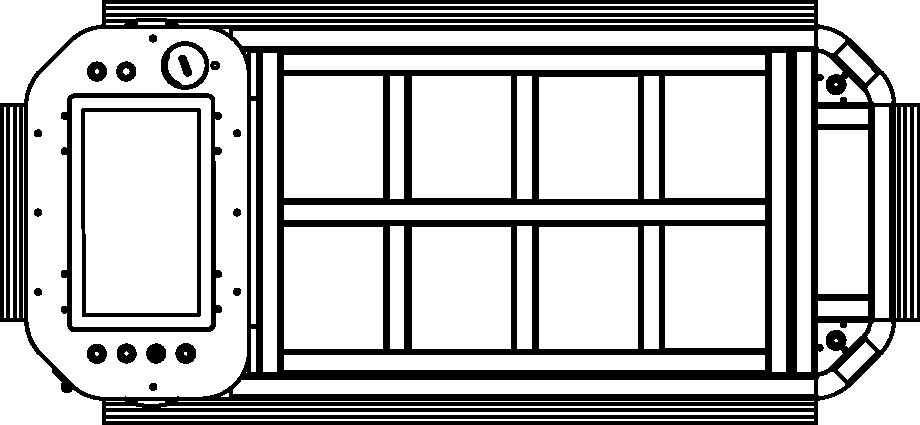
\includegraphics[width=0.9\textwidth]{Bilder/oben.pdf}
			\end{minipage}
			\begin{minipage}[b]{0.49\textwidth}
				(b)
				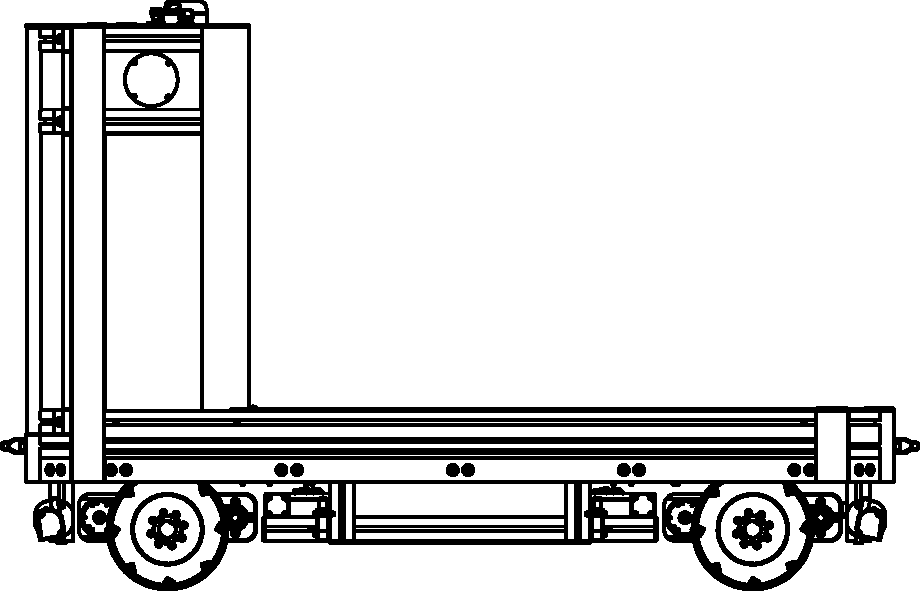
\includegraphics[width=0.9\textwidth]{Bilder/seite.pdf}
			\end{minipage}
			\centering
			\caption{(a) Darstellung des autonomen Logistik-Fahrzeugs aus der Draufsicht. Die acht benachbarten Rechtecke in der Mitte des Fahrzeugs stellen die Ladefläche des Fahrzeugs dar. (b) Darstellung aus der Seitenansicht. Oben links in der Abbildung ist der Schaltschrank zu sehen. Die Räder des Fahrzeugs befinden sich unten links und unten rechts in der Darstellung.}
			\label{fig: Darstellung des ALFs}
		\end{figure}
		
		Das autonome Logistikfahrzeug ALF ist ein solches Transportfahrzeug. Die Idee des ALFs ist es ein Fahrzeug zu entwickeln, das nach seiner Fertigstellung Logistikaufgaben am Standort der Hochschule Bochum lösen soll. Es dient im Labor für Antriebstechnik der Hochschule Bochum als Versuchs- und Entwicklungsplattform für praktische Anwendungen. Der Entwicklungsprozess stellt sich aus diversen Bachelor- und Masterarbeiten zusammen, die sowohl Hardware, als auch Softwareimplementierungen vorsehen. Bisher wurden zwei Abschlussarbeiten inklusive der praktischen Anwendung am ALF geschrieben. M.Sc. Dennis Hotze und M.Sc. Dominik Eickmann entwickelten in ihrem Masterprojekt das Fahrzeug und konnten Fahraufgaben ferngesteuert und manuell erledigen. Während der darauffolgenden Bachelorarbeit wurde eine Schlupfkompensation entwickelt, die den Drift am Fahrzeug durch Eingabe von Umgebungsinformationen verhindert. Weiterhin wurden Funktionen entwickelt, um grundlegende und autonome Fahraufgaben zu lösen. Das autonome Logistikfahrzeug aus der vorangegangenen Bachelorarbeit dient auch in dieser Masterarbeit als Versuchsplattform.\\
		
		Der tägliche Kontakt zu Menschen ist nicht nur für den ALF, sondern auch für andere Transportfahrzeuge im öffentlichen Raum unentbehrlich. Kreuzen sich die Wege eines autonomen Fahrzeugs mit der einer oder mehrerer Personen, darf es in keinster Weise zur Kollision kommen. Je nach Dimension des Fahrzeugs können die Folgen fatal sein. Das ALF zählt mit einem Maximalgewicht von 600 kg zu der Art von Fahrzeugen, die bei einem Zusammenstoß besonders schwere Verletzungen hervorrufen kann. Ein solches System muss folglich in der Lage sein, bei Annäherung von Personen eine gesonderte Gefahreneinschätzung vorzunehmen. Im Einsatz an der Hochschule Bochum kommt es eher selten zu Begegnungen mit Tieren ohne der Begleitung von Personen. Dementsprechend wird das System im Rahmen dieses Projekts auf die Erkennung von Personen beschränkt. Ein weiteres, übliches Szenario solcher Systeme im öffentlichen Raum ist die Bedienung durch nicht autorisierte Personen. Für derartige Zwecke muss ein Mensch nicht nur als bewegtes Objekt, sondern auch als solcher erkannt werden. \\
		
		Am ALF sind zwei \textit{Kinect}-Kameras angebracht \cite{Bachelorarbeit}. Bisher wurde der Großteil der Funktionen dieser Kameras nicht verwendet. In der vorangegangenen Bachelorarbeit wurden dreidimensionale in zweidimensionale Tiefeninformationen umgewandelt, um ein Problem bedingt durch die Einbauhöhe der Kameras zu lösen \cite{Bachelorarbeit}. Das Hauptziel dieser Masterarbeit ist die Entwicklung einer Personenerkennung. Die genannten Kameras dienen neben eines \textit{Light Detection and Ranging} (LiDAR) Sensors als einzige optische Sensoren des autonomen Logistikfahrzeugs. Zwar gibt es technische Lösungen für eine Personenerkennung mithilfe von zweidimensionalen Laserdaten. Jedoch werden Menschen mithilfe von Bildverarbeitung deutlich genauer detektiert. Folglich wird das System zur Personenerkennung mithilfe der beiden \textit{Kinect} Kameras ausgelegt. Weiterhin soll das System nicht nur Personen detektieren können, sondern diese auch wiedererkennen. \\
		
		Während der Bearbeitung von Transport- oder Fahraufgaben eines autonomen Fahrzeugs kann es zu diversen Komplikationen kommen. Beispielsweise können besonders im Anwendungsbereich der Hochschule Bochum diverse Objekte den Verlauf einer Route unterbrechen und ein Ziel sogar unerreichbar machen. Häufig können diese Probleme durch menschliche Hilfe beseitigt werden. Wiederum setzt dies eine Interaktion mit umstehenden Personen vorraus. Eine Besonderheit dieser Masterarbeit ist die theoretische und praktische Entwicklung parallel zu einem weiteren Projekt. Hannes Dittmann entwickelt in seiner Masterarbeit eine Sprachverarbeitung zur Klassifikation anwendungsorientierter Sprache \cite{Dittmann}. Diese stellt eine auditive \textit{Mensch-Maschine-Interface} (MMI) Schnittstelle her. So kann eine Person über ein Aufnahmegerät mit dem System kommunizieren. Die klassifizierte Sprache ist ohne Weiteres nicht in der Lage das Fahrzeug enstprechend zu steuern.\\
		
		Demnach wird in dieser Masterarbeit ein Konzept zur Steuerung des ALFs mit klassifizierter Sprache entwickelt und am Fahrzeug implementiert. Darüber hinaus gilt es die Steuerung des Systems nach gegebenen Standards auszulegen. Die \textit{Society of Automotive Engineers} (SAE) ist eine Organisation, die aus über 128000 Ingenieuren und technischen Experten besteht \cite{saeorg}. Ziel dieser ist im Allgemeinen die Weiterentwicklung im Thema Mobilität \cite{saeorg}. Unter anderem veröffentlicht \textit{SAE International} Normen, wie die \textit{SAE J3016}. Diese beschäftigt sich mit verschiednen Stufen der Automatisierung von Fahrzeugen. Eine entsprechende Tabelle ist in Abbildung \ref{fig: tabautonom} dargestellt.\\
		
		Das ALF wird zum Zeitpunkt des Entwicklungsbeginns dieser Masterarbeit auf dem \textit{SAE-Level} 3 eingeschätzt. Hierbei werden lediglich die autonomen Fahrmodi des Fahrzeugs berücksichtigt. Die Fahrbefehle konnten selbstständig durch das System ausgeführt werden und die Umgebung über die bereits genannten, zweidimensionalen Laserdaten erfasst werden. Die \textit{Fallback Performance} beschreibt den Übergang des automatisierten oder autonomen in einen risikominimalen Zustand. Bisher musste die laufende Software des ALFs auch im Fehlerfall manuell am Fahrzeug beendet werden. Dies bestärkte die Einschätzung, dass das Fahrzeug bedingt automatisiert sei.	
		
		\newcolumntype{C}[1]{>{\centering\arraybackslash}p{#1}}
\newcolumntype{M}[1]{>{\centering\arraybackslash}m{#1}}
\begin{table}[H]
	\caption{Übersicht der sechs Automatisierungsstufen nach SAE Standard J3016. Die Angaben wurde von der Quelle übernommen und sind sinngemäß übersetzt. \cite{sae}  }
	\begin{center}
		\begin{tabular}{|M{10mm}|M{48mm}|M{20mm}|M{20mm}|M{15mm}|M{20mm}|}
			\hline
			SAE Level  & Name & Ausführung von Fahrbefehlen & Erfassung der Umgebung& Fallback Performance& System-auswirkung\\ \hline
			\multicolumn{6}{|c|}{Benutzer überwacht die Fahrumgebung}\\ \hline
			
			0	& Keine Automatisierung			&Benutzer   &Benutzer &Benutzer & k.A.	 \\ \hline
			1	& Assistiert					& Benutzer \& System &Benutzer &Benutzer & Einige Fahrmodi	 \\ \hline
			2	& Teilautomatisiert				& System 	 &Benutzer&Benutzer&Einige Fahrmodi	 \\ \hline
			\multicolumn{6}{|c|}{Automatisiertes System - System überwacht Fahrumgebung}\\ \hline
			3	& Bedingte Automatisierung		& System &System&Benutzer&Einige Fahrmodi	 \\ \hline
			4	& Hochautomatisiert			& System &System&System&Einige Fahrmodi	 \\ \hline
			5	& Vollautomatisiert (autonom)	& System&System&System&Alle Fahrmodi	 \\
		
			
			\hline
		\end{tabular}
	\end{center}

	\label{fig: tabautonom}
\end{table}
		
		Als weiteres Ziel dieser Masterarbeit wird das ALF im Rahmen der technischen und sicherheitsrelevanten Möglichkeiten auf das \textit{SAE-Level} 5 angehoben. Dies betrifft insbesondere die zu entwickelnde Steuerung des Fahrzeugs.\\
		
		Diese und die Masterarbeit von Hannes Dittmann bilden im praktischen Kontext ein überarbeitetes Gesamtsystem des bereits bestehenden autonomen Logistikfahrzeugs. Die genannten Ziele sind im angehängten Lastenheft festgehalten und haben somit einen anwendungsorientierten Hintergrund. Der Anspruch an das zu entwickelnde System, ist die Zielerreichung mittels wissenschaftlicher Methoden zu erarbeiten.  
		
		
	